\documentclass[fullpage]{article}
\addtolength{\oddsidemargin}{-.875in}
\addtolength{\evensidemargin}{-.875in}	
\addtolength{\textwidth}{1.75in}

\usepackage{graphicx} 
\usepackage{amsmath}
\usepackage{caption}
\usepackage{listings}
\usepackage{xcolor}

\title{ESE461 Lab \#1 Report}
\author{Bryan Orabutt}

\begin{document}
\maketitle

\section*{Simulated Results}
For this lab I created several verilog files to implement different circuits. I used single unified testbench code to instantiate and test each of these circuits as a module. Figure~\ref{fig:results} shows the full simulated output from DVE.

\begin{figure}[ht!]
 	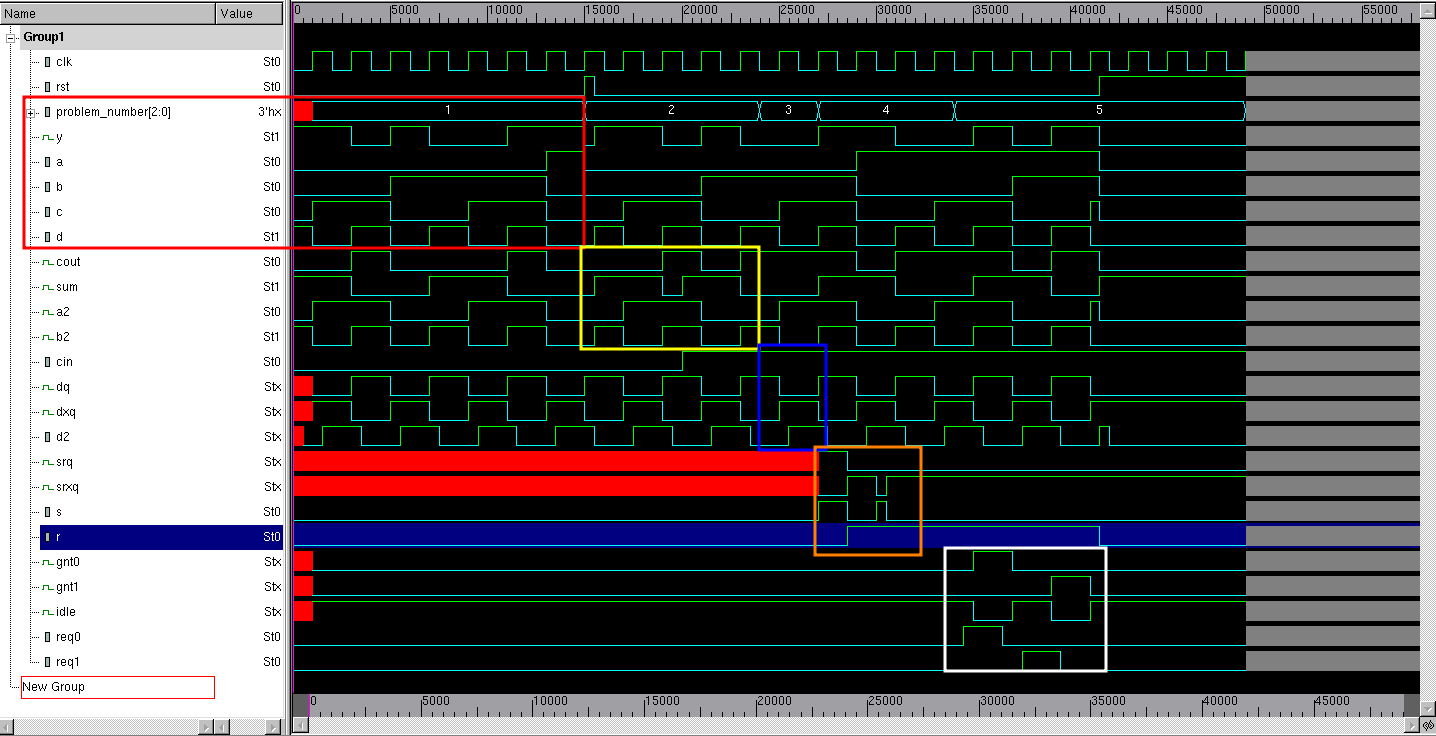
\includegraphics[scale=0.45,keepaspectratio=true]{../images/lab1.png}
 	\caption{Simulated waveforms for lab 1. Red shows the tests running for problem 1, yellow shows problem 2, blue shows problem 3, orange shows problem 4, and white shows problem 5.}
 	\label{fig:results}
\end{figure}

\section*{Problem 1}

For this problem I used data flow descriptions (i.e. assign statements) for each node of the circuit since it's a very simple combinational circuit described by: $y = a \oplus b \oplus c \oplus d$. Below figure~\ref{fig:p1} shows the output.

\begin{figure}[ht!]
 	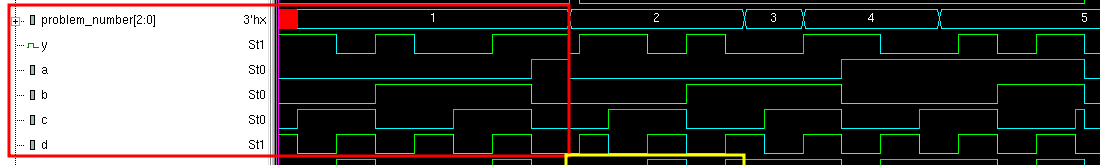
\includegraphics[scale=0.5,keepaspectratio=true]{../images/prob1.png}
 	\caption{Simulated waveforms for problem 1}
 	\label{fig:p1}
\end{figure}

As can be seen from the waveform data, the output \emph{y} only has a true output if exactly one of the inputs, \emph{a, b, c} or \emph{d} are true. If more than one input is true the output is false.

\section*{Problem 2}

Similar to problem 1, a simple full adder circuit is easiest to implement using data flow descriptions of the circuit. Figure~\ref{fig:p2} shows the output of my full adder circuit.

\begin{figure}[ht!]
 	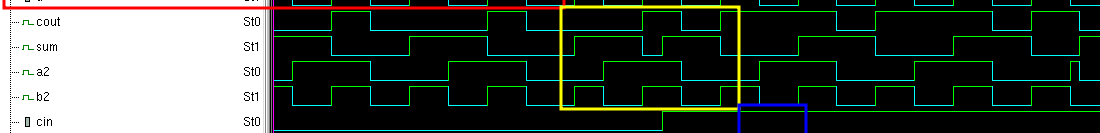
\includegraphics[scale=0.5,keepaspectratio=true]{../images/prob2.png}
 	\caption{Simulated waveforms for problem 2}
 	\label{fig:p2}
\end{figure}

The waveforms show that sum is false when all inputs are false, and true when any one of the inputs is true. Sum is also false if at least two inputs are true, but this makes cout true. Both cout and sum are true if all three inputs are true.

\section*{Problem 3}

This problem involved a sequential element: the D flip-flop. To implement this I chose to use a behavioral description of how a D filp-flop works. Figure~\ref{fig:p3} shows the simulation output.

\begin{figure}[ht!]
 	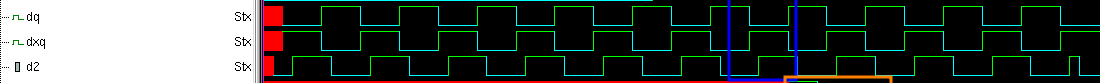
\includegraphics[scale=0.5,keepaspectratio=true]{../images/prob3.png}
 	\caption{Simulated waveforms for problem 3}
 	\label{fig:p3}
\end{figure}

To test this, I made an input called \emph{d2} which always transitions 5 ns after a clock edge. As can be seen by the simulated waveforms, when the clock edge comes, \emph{dq} follows \emph{d2} and \emph{xdq} is always the inverse of \emph{dq}.

\section*{Problem 4}

This problem specifically called for a structural description of an SR latch. The verilog code thus called NOR gate primitives to create a pair of cross coupled NOR gates and form an SR latch. Figure ~\ref{fig:p4} shows the simulation output for this problem.

\begin{figure}[ht!]
 	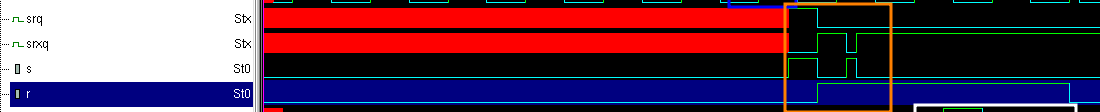
\includegraphics[scale=0.5,keepaspectratio=true]{../images/prob4.png}
 	\caption{Simulated waveforms for problem 4}
 	\label{fig:p4}
\end{figure}

Initially, both inputs are false so the outputs of the SR latch are in an undefined state. However, once I bring the S input high (while keeping R low) the \emph{srq} output shows a true value while the \emph{xsrq} shows false. This output does not change now unless I bring the R input high (leaving S low), in which case \emph{srq} becomes false and \emph{xsrq} becomes true.

\section*{Problem 5}

For this problem I wrote a behavioral description of the state machine described and depicted. I made use of a case statement to handle the combinational logic that determines the next sate, and an always block to assign the current state to next state every clock cycle. Figure~\ref{fig:p5} shows the simulation output.

\begin{figure}[ht!]
 	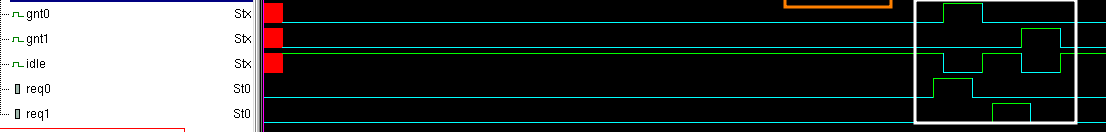
\includegraphics[scale=0.5,keepaspectratio=true]{../images/prob5.png}
 	\caption{Simulated waveforms for problem 5}
 	\label{fig:p5}
\end{figure}

The circuit is in an undefined state initially until the first cycle throws it into the IDLE state. The machine goes into the GNT0 state if \emph{req0} is asserted, and stays there as long as it remains asserted. If \emph{req0} is de-asserted then the machine returns to IDLE. The machine enters the GNT1 state if it is IDLE and \emph{req1} is asserted, and stays there as long as it remains asserted. Once it is de-asserted the machine returns to IDLE on the next clock edge.

\section*{Code}
\lstset{
         language=Verilog,
         basicstyle=\scriptsize\ttfamily,
         emptylines=0, 
         lineskip=1pt,
         %numbers=left,            
         numberstyle=\tiny,         
         stepnumber=2,              
         numbersep=5pt,             
         tabsize=3,                
         extendedchars=true,       
         breaklines=true,            
         commentstyle=\color{blue},
         keywordstyle=\color{red},
            frame=b,         
 %        keywordstyle=[1]\textbf,    
 %        keywordstyle=[2]\textbf,    
 %        keywordstyle=[3]\textbf,  
 %        keywordstyle=[4]\textbf,   \
         stringstyle=\scriptsize\color{green}\ttfamily, 
         showspaces=false,         
         showtabs=false,            
%         xleftmargin=17pt,
%         framexleftmargin=17pt,
%         framexrightmargin=5pt,
%         framexbottommargin=4pt,
         %backgroundcolor=\color{lightgray},
         showstringspaces=false           
 }
\subsection*{Problem 1}
\lstinputlisting{../problem1.v}

\subsection*{Problem 2}
\lstinputlisting{../problem2.v}

\subsection*{Problem 3}
\lstinputlisting{../problem3.v}

\subsection*{Problem 4 }
\lstinputlisting{../problem4.v}

\subsection*{Problem 5}
\lstinputlisting{../problem5.v}

\subsection*{Testbench}
\lstinputlisting{../lab1_tb.v}

\end{document}
